% \setcounter{chapter}{3}
\chapter{Chapitre 2 - L'analyse multidimensionnelle par réseau de co-expression de gènes}
% \chapter*{Chapitre 2 - L'analyse multidimensionnelle par réseau de co-expression de gènes}
% \phantomsection\addcontentsline{toc}{chapter}{Chapitre 2 - À définir} 
%%\chapter{Titre du chapitre}     % numéroté
\label{chapter:multidim}

La variation de la distribution de la co-expression des gènes associée au vieillissement est une propriété qu'on a pu observer dans le muscle lors du chapitre précédent. Grâce à elle, on a pu isoler dans le chapitre précédent des gènes dont la fonction biologique est confirmée comme liée au vieillissement du muscle. On peut alors considérer l'étude de la topologie des réseaux de co-expression de gènes comme une méthode efficace pour la détection de gènes biomarqueurs du vieillissement dans un tissu. 

Cependant le vieillissement est un phénomène qui ne se limite pas au muscle dans un organisme et touche bien d'autres tissus en parallèle. Dans chacun d'eux, le transcriptome est le témoin des modifications liées à l'avancée dans l'âge. Comme souligné en introduction (voir \ref{intro_biomarker_aging}), l'analyse d'expression différentielle ainsi que d'autres méthodes d'analyse de gènes discrètes \cite{Barabasi2004} ont permis de relever nombre de gènes (biomarqueurs) associés à l'âge et de créer des bases de données les regroupant. 

Si certains de ces gènes ont déjà vu étudié les liens les unissant dans des fonctions physiologiques, ce n'est pas le cas de la majorité. Ce manque est dû aux méthodes longues et/ou couteuses d'obtention de ces informations qui requièrent notamment des expérimentation basées sur des inactivation ou sur-activation \todo{La traduction dans le grand dico du québec c'est "invalidation" mais y'a rien pour knock in. Et puis c'est moins parlant je trouve.} d'un ou plusieurs gènes (respectivement \textit{knockout} et \textit{knockin} en anglais). 
L'information apportée par de tels liens permettrait pourtant d'aider à déterminer le type de modification observé \cite{Lopez-Otin2013} : l'activation/répression du gène observé est-elle le fruit d'une réponse à l'activation d'un autre gène voir mécanisme complet ? Ou bien est-elle à l'origine d'un mécanisme justement, avec ou sans autres gènes impliqué ? 

Ces questions (qu'on peut résumer à "conséquence ou cause") ont d'autant plus d'intérêt que des études précédentes tendent à démontrer l'existence de bases communes au vieillissement (fonctions physiologiques et mécanismes) \cite{DeMagalhaes2009a}. On relève ainsi des signatures d'expression de gènes communes à plusieurs tissus dans leur état "âgé". Parmi les fonctions physiologiques détectées comme sur-exprimées par l'expression différentielle, on retrouve notamment des composantes de la réponse immunitaire/inflammatoire et de la dégradation lysosomale. À l'opposé, dans les fonctions détectées comme sous-exprimées, on retrouve des fonctions associées à l'encodage de protéines mitochondriales ainsi que des gènes responsables de la production de différents types de collagène. En complément, bien que n'étant pas commun à tous les tissus du corps, d'autres signatures sont communes à des sous groupes de tissus partageant des propriétés : accumulation de marques de réparation de l'ADN chez les tissus se renouvelant rapidement \cite{Armanios2012}, épuisement des capacités de régénération chez les tissus disposant d'une cache de cellules souches \cite{Ratajczak2017}, dommages à l'ADN plus présents chez les tissus soumis à des stress mécaniques \cite{Kubben2017}, etc.

L'analyse de co-expression de gènes ayant déjà démontré sa capacité à aider à la détermination de nouveaux liens, de nouvelles voies de signalisation dans un tissu \cite{Hughes2000}, on souhaite l'employer pour créer des liens entre tissus. Dans ce chapitre, on s'attachera donc à déterminer si l'analyse par réseaux de co-expression de gènes permet de répondre à ce besoin \todo{Peut etre reformuler pour que ça fasse plus hypothès/problématique}. On commencera par traiter les données issues de différents tissus tout en expliquant les précautions prises, on poursuivra par l'exploration générale des modules de gènes obtenus, et enfin on s'attardera sur les apports du croisement de données entre modules modérément et/ou non préservés. \todo{Reverifier plus tard si ce plan tient toujours, notamment si on a pas rajouté un aspect etude de la déconnexion}

% Objectif principal : 
% Étudier la variation de la déconnexion entre les tranches d'âge extrêmes 
% dans de multiples tissus

% Objectifs secondaires :

% * Vérifier le nombre d'échantillons par tranche d'âge de 10 ans
% * Identifier les tissus d'intérêt pour explorer la déconnexion.
% * Détecter les modules avec chute de connectivité.
% * Déterminer les gènes communs et les gènes spécifiques, et leurs interactions.
% * Explorer les modèles de déconnexion entre les tissus.

\section{Données et pré-traitement}

\subsection{Description des données}

Comme dans le chapitre \ref{chapter:gwena}, on a utilisé les données issues de l'étude GTEx \cite{Ardlie2015}. Pour aller plus en détail que ce que ne le permet le format d'article du chapitre \ref{chapter:gwena}, ces données sont le regroupement d'échantillons prélevés sur 54 tissus (+1 tissu qui est en fait un assemblage de lignées cellulaires dérivées de patients atteints de leucémie myéloïde aiguë\cite{Way2020}) et 948 donneurs dans sa dernière version, la v8 (Table \ref{table:gtex_sample_tissues_donnor}. Cette variété de tissus vise à être le plus représentatif possible (au vu du coup de prélèvement et d'analyse de chaque échantillon) des différents tissus chez l'humain. Les biopsies sont effectuées sur des donneurs décédés (avec leur accord préalable, l'accord d'un proche, ou l'accord du représentant légal) dans 4 centres de collecte, puis analysées sur place ou transférées selon le tissu avec réfrigération durant le transport. Ces échantillons sont évalués sur plusieurs critères pour jauger leur admissibilité : des critères cliniques (absence de contamination au VIH, absence de chimiothérapie dans les 2 ans, absence de transfusion sanguine dans les 48h, etc.), des critères anatomopathologiques (absence de tissu cancéreux, absence de pathologie tissulaire, etc.) et des critères analytiques (quantité de tissu prélevé suffisante, quantité d'ARN extrait final supérieur à 500ng d'ARN total, nombre d'intégrité d'ARN ou RIN supérieur à 5.7) \cite{Carithers2015}. Tout échantillon non conforme est exclu de la cohorte.

Sur la majorité intégralité des échantillons ont été effectué des séquençages de génome (\textit{Whole Genome Sequencing}, WGS), des séquençages d'exome complet (\textit{Whole Exome Sequencing}, WES), des séquençage de transcriptome (aussi appelé séquençage d'ARN, RNA-Seq), ainsi que des des images de coupes histologiques colorées. Des données reformatées sont également mises à disposition telle que les locus de caractères quantitatifs (\textit{quantitative trait loci}, QTL) et l'expression de gène qui est ce que l'on va utiliser ici. Ces données sont disponibles sur le site du consortium GTEx (\url{https://gtexportal.org}) accompagnées d'information sur le phénotype des échantillons. En raison du fort potentiel d'identification des donneurs, le phénotype donné publiquement est partiel, et le phénotype complet est disponible sur demande auprès de dbGaP après soumission d'un dossier de projet à renouveler chaque année (Annexe \ref{annexe:dbgap}).

\begin{table}[h]
\centering
\begin{tabular}{llll}
\textbf{GTEx V8} & \textbf{\# Tissus} & \textbf{\# Donneurs} & \textbf{\# Échantillons} \\ \hline
Total            & 54                 & 948                  & 17382                    \\
Avec Genotype    & 54                 & 838                  & 15253                    \\
Avec eQTL        & 49                 & 838                  & 15201                   
\end{tabular}
\caption{Nombre de tissus, donneurs et échantillons disponibles selon les données}
\label{table:gtex_sample_tissues_donnor}
\end{table}

Par ailleurs, tous les donneurs ne peuvent pas être prélevés pour l'ensemble des 54 tissus et ce sont en moyenne 23,4 tissus qui sont prélevés (v8). Certains tissus ont par ailleurs été priorisés lors des biopsies : tissu adipeux (sous-cutané), artère tibiale, coeur (ventricule gauche), poumon, muscle (squelettique), nerf tibial, peau (exposée au soleil), thyroïde, sang complet. Parmi les différents tissus biopsiés, il est à noter que certains sont issus d'un même organe et on a ainsi 31 organes biopsiés pour 54 tissus biopsiés en tout (Figure \todo{faire une figure avec cette info}).

\todo[inline]{Un Sankey diagramme des tissus avec col 1 = SMTS, col 2 = SMTSD, col 3 = tranche d'age à 10 ans}


\subsection{Sélection des tissus}

\todo[inline]{Faire une figure avec l'évolution de la disparition du nombre de tissus}

Le vieillissement est un phénomène dont les altérations moléculaires sont linéaires avec le temps, dont les dommages cellulaires sont super-linéaires \cite{Todhunter2018}, et où la mortalité associée augmente de façon exponentielle passé 20 ans \cite{Finch2016}. Afin de faciliter la détection de ces altérations grâce à l'analyse de co-expression différentielle, on s'est donc dans un premier temps concentré sur une sélection de tranches d'âges très contrastées. Les échantillons sélectionnés sont issus de donneurs entre 20 et 30 ans pour la tranche qu'on nommera "jeune", et entre 60 et 70 ans pour la tranche qu'on nommera "âgée". Les données de GTEx ne comportent toutefois pas un nombre d'échantillons similaire pour chacune de ces tranches du fait de la mortalité plus importante chez les personnes âgées que les personnes jeunes (principalement des décès par traumatisme chez les jeunes plutôt que par maladie chronique ou maladie liée à l'âge chez les âgés). Un premier filtre de notre pré-traitement restreint donc la sélection des tissus à ceux comportant au minimum 50 échantillons dans chacune des tranches d'âge, ce qui n'est pas le cas de la Vessie (20) et le Rein - Médulla (3). Ce nombre d'échantillons permet d'assurer un bon compromis entre des réseaux de co-expression de gènes robustes (donc non sensibles à des valeurs aberrantes) et la perte de plus de tissus à étudier dans cette analyse multidimensionnelle qu'on souhaite effectuer \cite{Liesecke2019}.

Par ailleurs, tous les tissus restant n'étaient pas nécessairement adaptés à l'étude globale du vieillissement chez l'humain. Ainsi on a retiré tous les tissus liés à un seul sexe : Trompes de Fallope, Col de l'utérus, Utérus, Vagin, Sein, Ovaire, Prostate, Testicule. À ce retrait s'ajoute celui des échantillons de lignées cellulaires (dérivées ou non de tissus eux concervés) car non représentatifs du vieillissement biologique : Cellules - Lymphocytes transformés par EBV, Cellules - Fibroblastes cultivés, Cellules - Lignée cellulaire de leucémie (CML). 


\begin{figure*}[h]
    \centering
    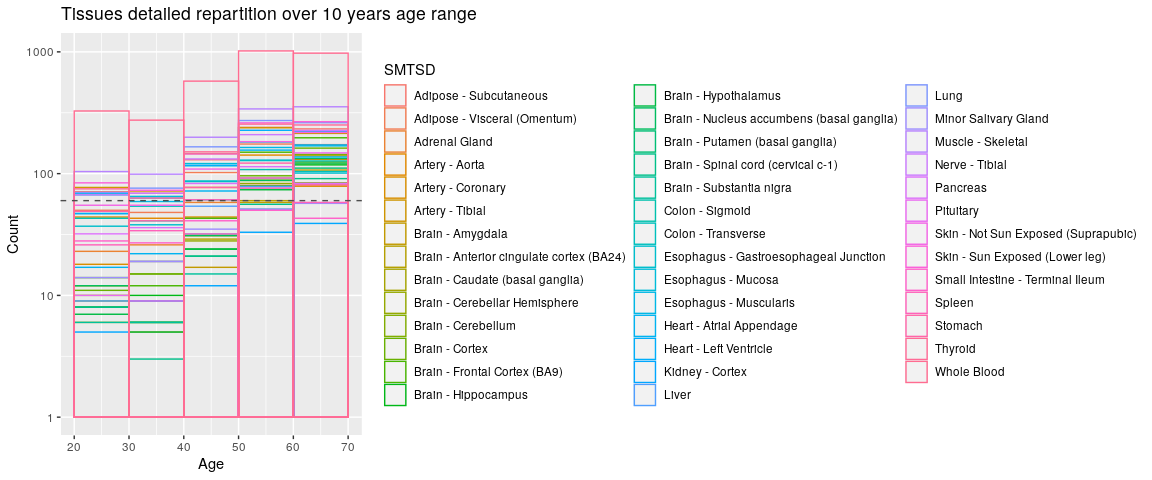
\includegraphics[width=1\textwidth]{img/chap2/chap2_sample_count_by_tissu.png}
    \label{figure:sample_count_by_tissu}
    \caption{Nombre d'échantilllons disponibles par tissu et par tranche d'âge de 10 ans dans les données de GTEx.}
\end{figure*}


\subsection{Filtre des échantillons}

\todo[inline]{Faire une figure avec l'évolution de la disparition du nombre d'échantillons. Ou bien faire du 2 en 1 avec la précédente sur les selections de tissus ?}

En plus de ces sélections de tissus, certains échantillons ont directement nécessité une filtration afin de prévenir de potentiels biais. Ainsi, seuls les échantillons répondant au critère d'inclusion dans la cohorte "GTEx Analysis Freeze" ont été retenus en premier lieu. Cette cohorte atteste que les échantillons n'étaient pas issus de donneurs ayant des liens de parenté ou de donneurs avec des critères d'exclusion, par exemple des donneurs avec des duplications/déletions chromosomiques, affectés d'un syndrome tel que défini par la base de données OMIM \cite{Hamosh2005} (ce qui n'inclue pas les maladies liées au vieillissement), ou encore ayant effectué une chirurgie de ré-assignation sexuelle. 

Par ailleurs, l'expression des tissus tumoraux a montré, dans des études préalables, des modèles d'expression génétique différents de ceux non tumoraux \cite{Tang2017}. Par conséquent, les échantillons de ces donneurs on également été supprimées ici ainsi que les échantillons dont le statut cancéreux était inconnu. 


\subsection{Correction des facteurs confondants}

À l'instar de l'analyse d'expression différentielle, l'analyse de co-expression différentielle nécessite des données biaisées au minimum pour une construction de réseau de qualité. Ces biais (ou facteurs confondants) peuvent être tant techniques que biologiques et vont entraîner une augmentation de la variation de façon artificielle. Le risque est alors de détecter une différence artificielle et de l'assumer comme expérimentalement pertinente alors qu'elle est en fait due aux biais. Dans le cas de la co-expression plus spécifiquement, ces bais peuvent entraîner des corrélations erronées mais qui semblent crédibles entre certains gènes. Elles altèrent alors la construction du réseaux de co-expression et par la suite la détection des modules qui se base sur un découpage en modules via les corrélations. Ainsi, il est essentiel de corriger ces facteurs confondants au préalable de l'utilisation du package R GWENA \todo{REF} sur les données comme on va le faire par la suite.

La complexité de la correction des facteurs confondant réside dans leur suppression sans pour autant altérer la distribution des données ou supprimer le signal expérimental d'intérêt, ici les variations dans le transcriptome dûs à l'âge. Il est également important avec l'utilisation de GWENA de veiller à ce que la correction n'altère pas la topologie d'invariance d'échelle qu'on retrouve dans les données de transcriptomique après construction d'un réseau de co-expression. En effet, cela invaliderait la méthode de détection des modules.
% Comme précisé en \ref{subsubsection:microarray_props_and_normalisation} et \ref{subsubsection:rnaseq_props_and_normalisation}, chaque technologie de séquençage a un premier ensemble de normalisations spécifique à elle, limitant ainsi un premier ensemble de biais spécifiques. 
\todo{Je me demande si ces 2 paragraphes plus haut ne devraient pas finir en \ref{chapter:intro}}

La base de données GTEx n'échappe pas aux biais et a même été étudiée sur le plan de la contamination \cite{Nieuwenhuis2020}.
Malgré le progrès de techniques ciblées sur des facteurs confondants connus comme l'effet de lot, l'effet de centre de prélèvement, le sexe, le poids, etc., celles-ci ne sont pas capables de corriger pour des facteurs peu explicites ou diffus comme la classe sociale, l'alimentation, la façon de manipuler des techniciens, etc. La correction par composante principale (CP) vise à répondre à ce type de problématique et a montré de bons résultats selon une évaluation par validation de pathways au sain de modules détectés. \cite{Parsana2019}. Elle a également montré de meilleurs résultats que d'autres méthodes telles que que la régression multiple, le taux exonique, ou encore le numéro d'intégrité d'ARN (\textit{RNA integrity number}, ou RIN). Fait important pour la co-expression en particulier, cette méthode conserve la propriété d'invariance d'échelle des données.

Cependant cette correction va également corriger pour notre variable d'intérêt, l'âge, si utilisée telle quelle. Pour conserver cette information tout en ayant un effet de correction par CP suffisant, on a donc ajusté la méthode pour ne retirer que les $n$ PC par tissu les plus corrélés à l'âge et retirant le moins de gènes corrélés à l'âge. Le nombre $n$ de PC à éliminer a été estimé en calculant la perte de corrélation entre le phénotype et l'expression des gènes et confirmé en recherchant le nombre de gènes significativement corrélés avec deux bases de données de gènes du vieillissement (Table \ref{table:nb_PC_corr_and_samples_by_tissue}) : GenAge \cite{DeMagalhaes2004} et Digital Aging Atlas \cite{Craig2015}.

\begin{table}[h!]
% \resizebox{\textwidth}{!}{
\centering
\begin{tabular}{llll}
\multirow{2}{*}{\textbf{Tissu}} & \multirow{2}{*}{\textbf{\begin{tabular}[c]{@{}l@{}}Nombre de CP \\ corrigées\end{tabular}}} & \multicolumn{2}{l}{\textbf{Nombre d'échantillons}} \\ \cline{3-4} 
                                &                                                                                             & \textbf{Jeune}            & \textbf{Âgé}           \\ \hline
Adipeux sous-cutané             & 1                                                                                           & 58                        & 227                    \\
Artère tibiale                  & 3                                                                                           & 65                        & 206                    \\
Muqueuse œusophagienne          & 1                                                                                           & 59                        & 160                    \\
Muscle œusophagien              & 3                                                                                           & 64                        & 138                    \\
Muscle squelettique             & 5                                                                                           & 73                        & 281                    \\
Nerf tibial                     & 4                                                                                           & 56                        & 219                    \\
Peau non exposée au soleil      & 4                                                                                           & 50                        & 220                    \\
Peau exposée au soleil          & 3                                                                                           & 65                        & 250                    \\
Thyroïde                        & 3                                                                                           & 53                        & 227                    \\
Sang complet                    & 1                                                                                           & 73                        & 259                   
\end{tabular}
% }
\caption{Résumé du nombre de composantes utilisées pour effectuer la correction de l'expression par tissu, ainsi que le nombre d'échantillons inclus dans chacun pour les deux plages d'âge.}
\label{table:nb_PC_corr_and_samples_by_tissue}
\end{table}

\todo[inline]{Idée de figure : remplacer cette table ou en touts cas la partie nb composantes par un ensemble de mini histogrames avec les deux bdd en un, et en facet pour chaque tissu.}

\subsection{Filtre sur les gènes}




\section{Construction des réseaux par tissu et détection des modules}



\begin{itemize}
    \item Tissu sanguin non exploitable
    \item 10 tissus exploitables
    \item 
    
\end{itemize}

\begin{table}[h]
\resizebox{\textwidth}{!}{
\begin{tabular}{llllll}
\textbf{}            & \textbf{Preserved} & \textbf{Moderately preserved} & \textbf{Unpreserved} & \textbf{Inconclusive} & \textbf{Total} \\ \hline
Adipeux sous-cutané & 12                 & 4                             & 0                    & 2                     & 18             \\
Artère tibiale        & 13                 & 8                             & 1                    & 1                     & 23             \\
Muqueuse œusophagienne     & 3                  & 8                             & 1                    & 0                     & 12             \\
Muscle œusophagien & 9                  & 6                             & 0                    & 6                     & 21             \\
Muscle squelettique      & 14                 & 13                            & 5                    & 3                     & 35             \\
Nerf tibial         & 35                 & 9                             & 1                    & 4                     & 49             \\
Peau non exposée au soleil & 36                 & 4                             & 0                    & 0                     & 40             \\
Peau exposée au soleil     & 10                 & 8                             & 2                    & 1                     & 21             \\
Thyroïde              & 12                 & 8                             & 1                    & 4                     & 25            
\end{tabular}
}
\caption{Nombre de modules par tissu et leur répartition selon leur statut de préservation.}
\label{table:modules_status_all_tissues}
\end{table}



% Idées :
% \begin{itemize}
%     \item Rajout d'information protéique pour "consolider" le réseau ?
%     \item Rajout d'une méthode de réseau consensus à GWENA ?
%     \item Differential co-expression avec un autre tissu sur lequel on peut avoir des jeux de données jeune/vieux pour récup les genes communs au vieillissement, ceux specifique à un tissu ou l'autres, et ceu combinant le vieillissement specifique au tissu ?
%     \item Une étude de l'impacte de la filtration sur l'état du réseau final ? Il n'y a rien de systemique dans la littérature, personne qui en fasse une review. Parsana et al. (alexis battle team) a fait ça en 2019 pour tester la PC-correction uniquement. Ils ont simulé des données scale free + des données scale free mimiquant GTEx et essayé de déterminer l'impact en calculant un FDR
% \end{itemize}










Tous les donneurs n'ont toutefois pas pu être prélevés pour l'ensemble des 54 tissus, entraînant une première disparité dans les données.

